\graphicspath{{4_chapter/figures/}}

% Define filter for appendix references, cf. https://tex.stackexchange.com/a/617196
% Ensure appendix references only contains references that do not appear in the main text
\defbibfilter{appendixOnlyFilter}{
    segment=1 % Segment 1 will be chosen to be the one in appendix
    and not segment=0 % Default segment is 0
}
% Use symbol for acknowledgements footnote
\renewcommand*{\thefootnote}{\fnsymbol{footnote}}
\chapter[Title of Chapter 3]{Title of Chapter 3\footnote{\noindent
This chapter is co-authored with Jane Doe. Acknowledgements here.}}
\label{chapter:chapter3-alias}
\markboth{Title of Chapter 3}{}
\newpage

% Move back to numbered footnotes and reset counter
\setcounter{footnote}{0}
\renewcommand*{\thefootnote}{\arabic{footnote}}

\section{\label{}Name of section}

This paper studies the macroeconomic effects of the increase wealth inequality using the framework of \citet{krusell1998income}. \lipsum[1-2]


\begin{figure}[htbp]
\centering
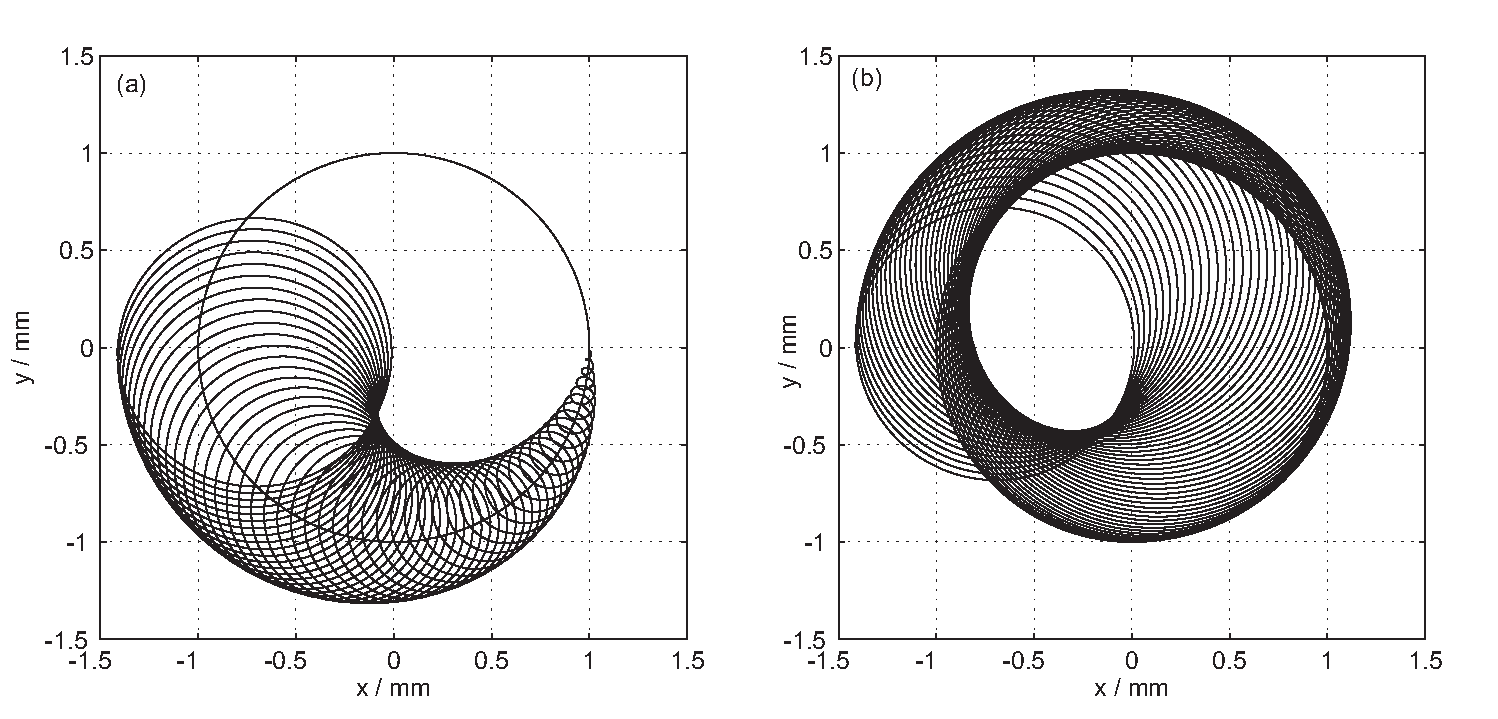
\includegraphics[width=\textwidth]{4_chapter/graphics/example}
\caption{\label{fig:chapter1-example}Example figure}
\begin{flushleft}
\emph{Notes.} Write here...
\end{flushleft}
\end{figure}


\lipsum[3-4]

\subsection{\label{}Name of subsection}

\lipsum[5-6]

\begin{table}[htbp]
\caption{Example Table}\label{tab:chapter3-example}
\centering
\begin{tabular}{lll}
        & Column 1 & Column 2   \\\hline
Row 1   & 1        & 2          \\
Row 2   & 3        & 4          \\\hline
\end{tabular}
\begin{flushleft}
\emph{Notes.} Write here...
\end{flushleft}
\end{table}


\lipsum[7-8]

\subsubsection{\label{}Name of subsubsection}

\lipsum[9-10]

\newpage{}
\printbibliography[segment=0,heading=subbibintoc]

\newpage{}
\begin{subappendices}
\newrefsegment %% <== increases the segment number (0 by default)
\begin{center}{\Large\textbf{Appendices}}\end{center}
\section{Appendix Section}

\lipsum[1-2] See also \citet{boppart2018exploiting}.

\newpage
\printbibliography[title=Appendix References,heading=subbibintoc,filter=appendixOnlyFilter]

\end{subappendices}
